This section summarizes how the experiments were conducted and their results.

\subsection{Methodology} \label{subsec:methodology}
Experiments were performed using the script \verb|jacobirun.sh|, as better explained in sub-section~\ref{subsec:runningexperiments}.
The script ran sequential, C++11 thread and FastFlow versions both on the Xeon CPU and Xeon Phi co-processor.
If executed on the Xeon CPU the number of workers for parallel versions went from $1$ to $16$, otherwise their number ranged from $1$ to $240$ (to match the number of contexts of the processor).
$N$, instead, assumed values of $5000$, $10000$, $15000$, and $30000$. 
Sadly bigger values of $N$ filled the memory of the co-processor, hence they were not included in the analysis.
All the tests of the FastFlow implementation used a fixed grain size of $10$.

\subsection{Results and remarks} \label{subsec:results}
Each of the graphs in this section reports experimental results in terms of efficiency, scalability, and speedup for each of the experiments described above.
\begin{figure}[h]
	\centering
	\begin{subfigure}[b]{0.3\linewidth}
		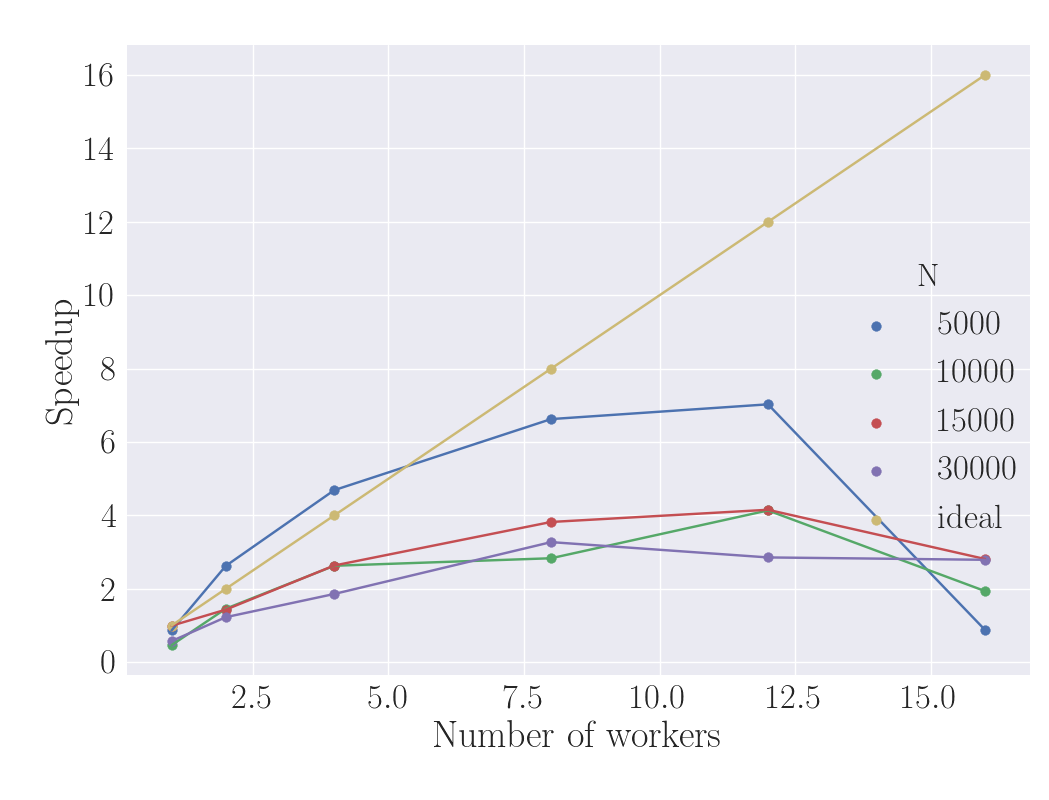
\includegraphics[width=\linewidth]{../graphs/graph_ff_host_s}
		\caption{Speedup graph.}
		\label{fig:ff_host_s}
	\end{subfigure}
	\begin{subfigure}[b]{0.3\linewidth}
		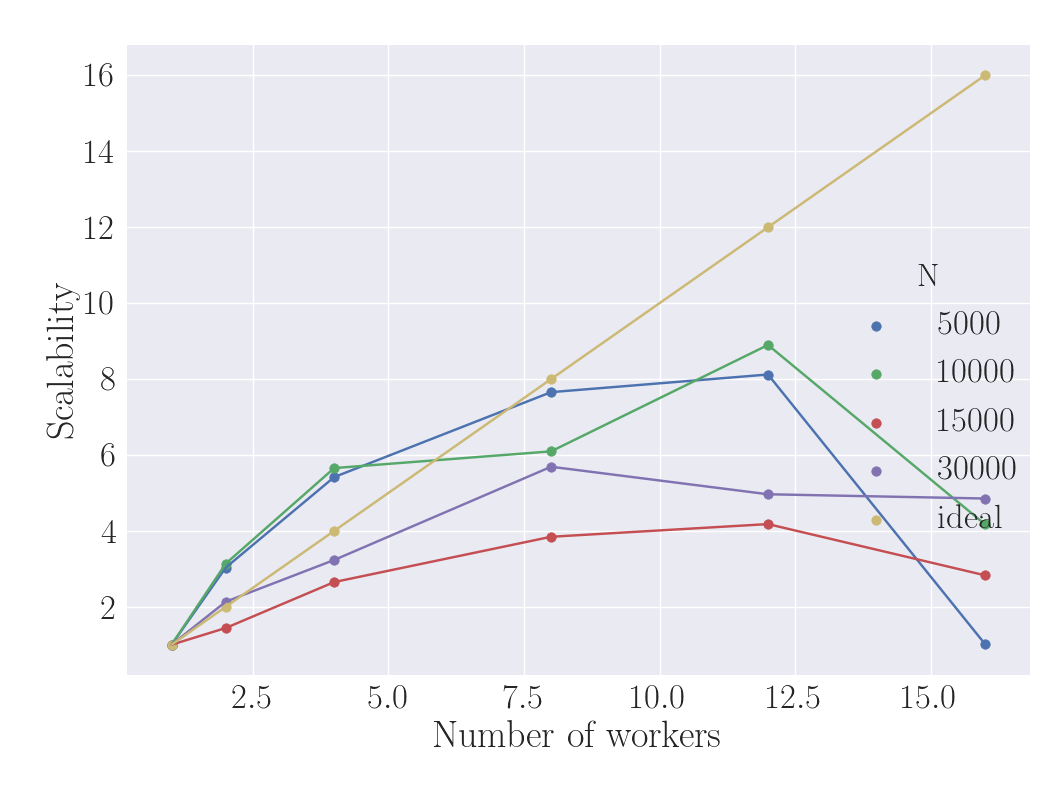
\includegraphics[width=\linewidth]{../graphs/graph_ff_host_scalab}
		\caption{Scalability graph}
		\label{fig:ff_host_scalab}
	\end{subfigure}
	\begin{subfigure}[b]{0.3\linewidth}
		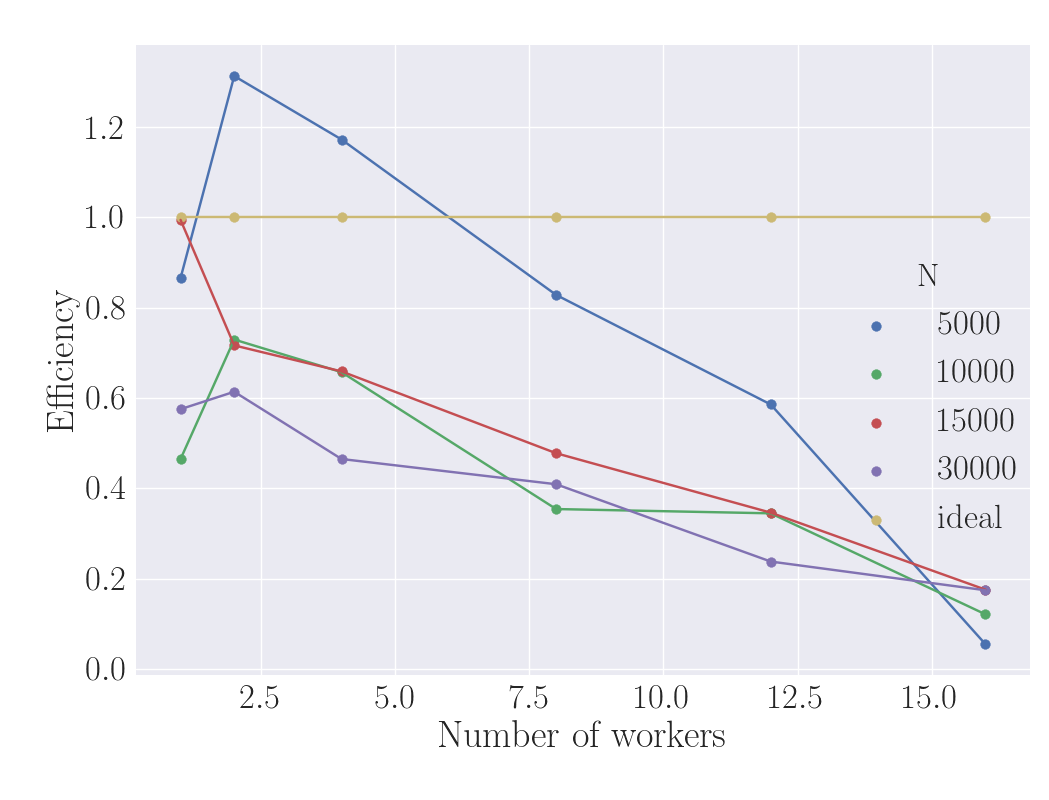
\includegraphics[width=\linewidth]{../graphs/graph_ff_host_eff}
		\caption{Efficiency graph}
		\label{fig:ff_host_eff}
	\end{subfigure}
	\caption{Graphs of different performance measures on the Xeon CPU using FastFlow. $N \in \{ 5000, 10000, 15000, 30000\}$}
	\label{fig:ff_host}
\end{figure}
~
\begin{figure}[h]
	\centering
	\begin{subfigure}[b]{0.3\textwidth}
		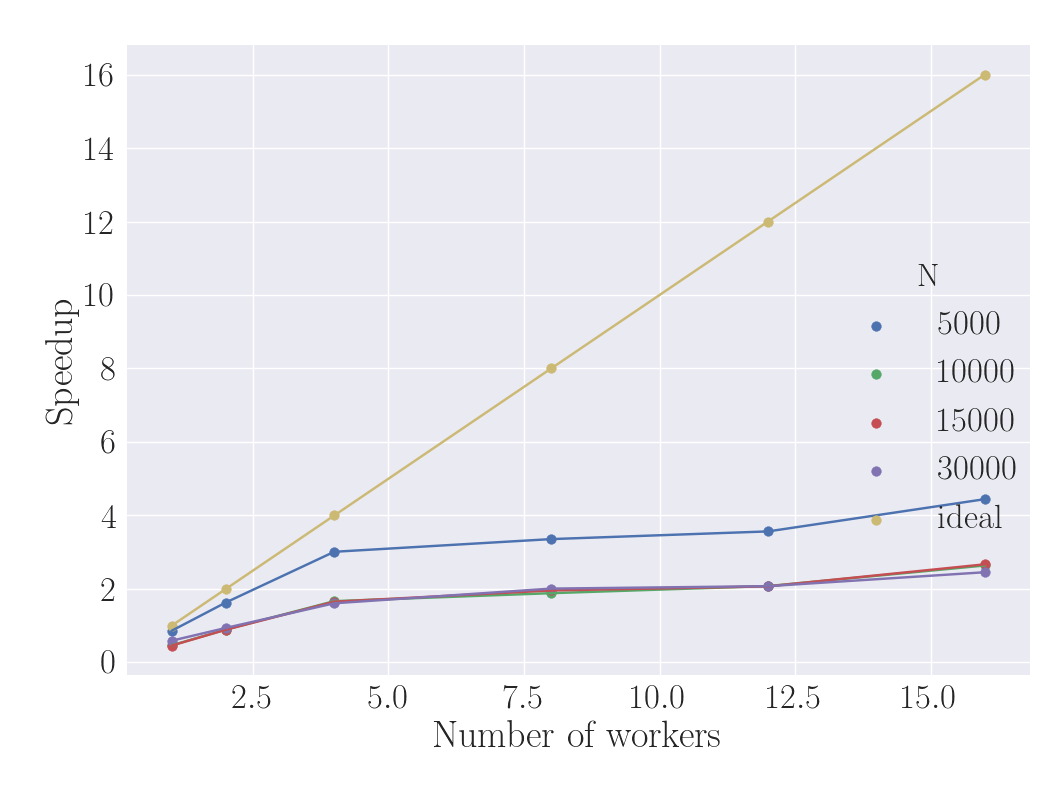
\includegraphics[width=\textwidth]{../graphs/graph_th_host_s}
		\caption{Speedup graph.}
		\label{fig:th_host_s}
	\end{subfigure}
	\begin{subfigure}[b]{0.3\textwidth}
		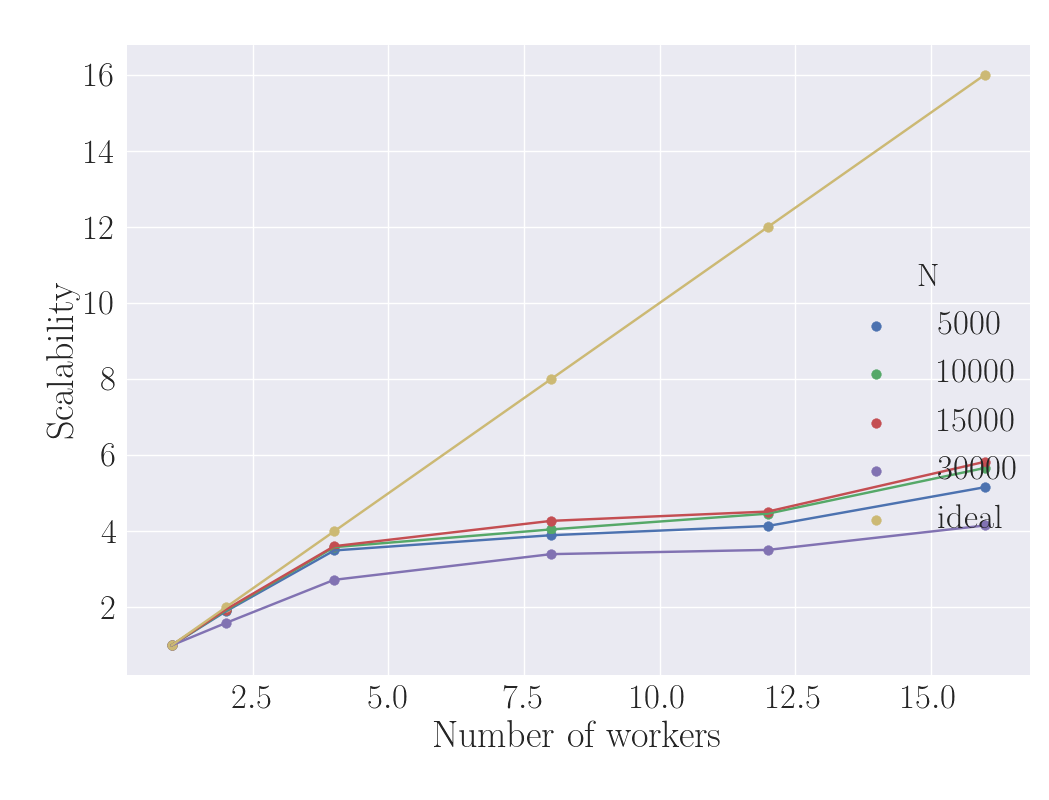
\includegraphics[width=\textwidth]{../graphs/graph_th_host_scalab}
		\caption{Scalability graph}
		\label{fig:th_host_scalab}
	\end{subfigure}
	\begin{subfigure}[b]{0.3\textwidth}
		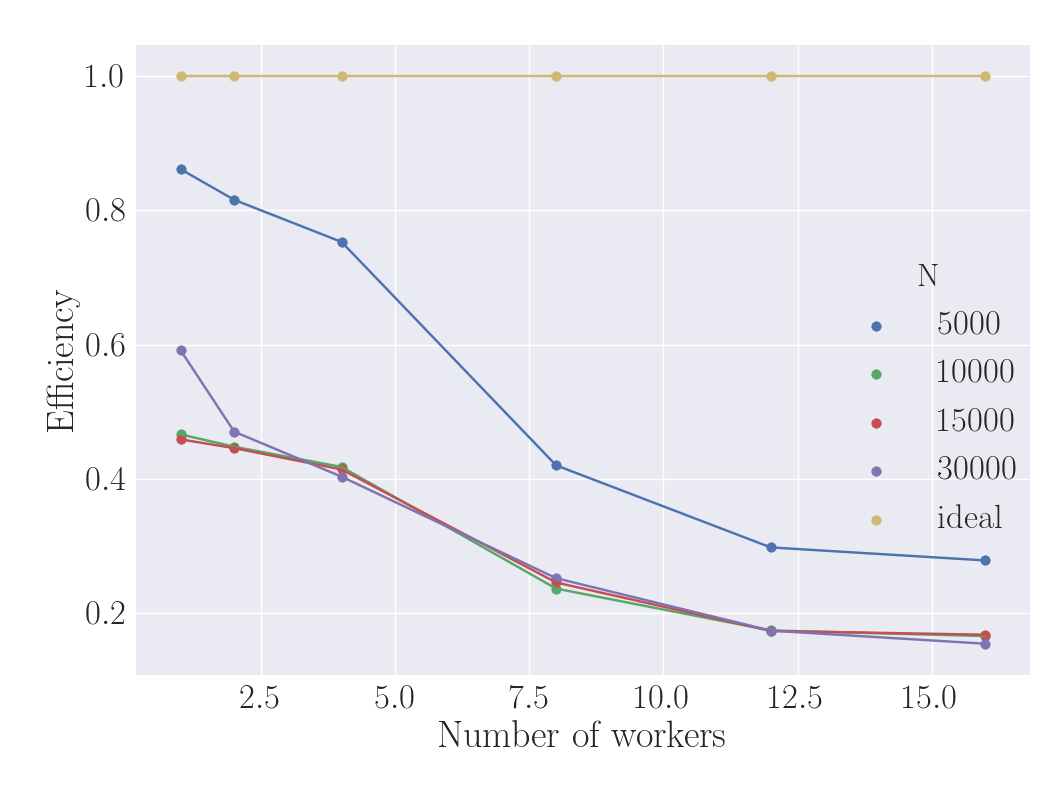
\includegraphics[width=\textwidth]{../graphs/graph_th_host_eff}
		\caption{Efficiency graph}
		\label{fig:th_host_eff}
	\end{subfigure}
	\caption{Graphs of different performance measures on the Xeon CPU using C++11 threads. $N \in \{ 5000, 10000, 15000, 30000\}$}
	\label{fig:th_host}
\end{figure}

Figure~\ref{fig:ff_host} and Figure~\ref{fig:th_host} respectively report the results of the execution of the FastFlow and C++11 thread implementation on the Xeon CPU.
It is interesting to see that none of the measured metrics adhere to the ideal curve, especially for bigger values of $N$.

Smaller values of $N$ had slightly to better w.r.t.\ bigger values of $N$, especially as the number of workers increased.
This is probably due to the fact non-negligible time is spent in cache coherence procedures for bigger values of $N$.

\begin{figure}[h]
	\centering
	\begin{subfigure}[b]{0.3\textwidth}
		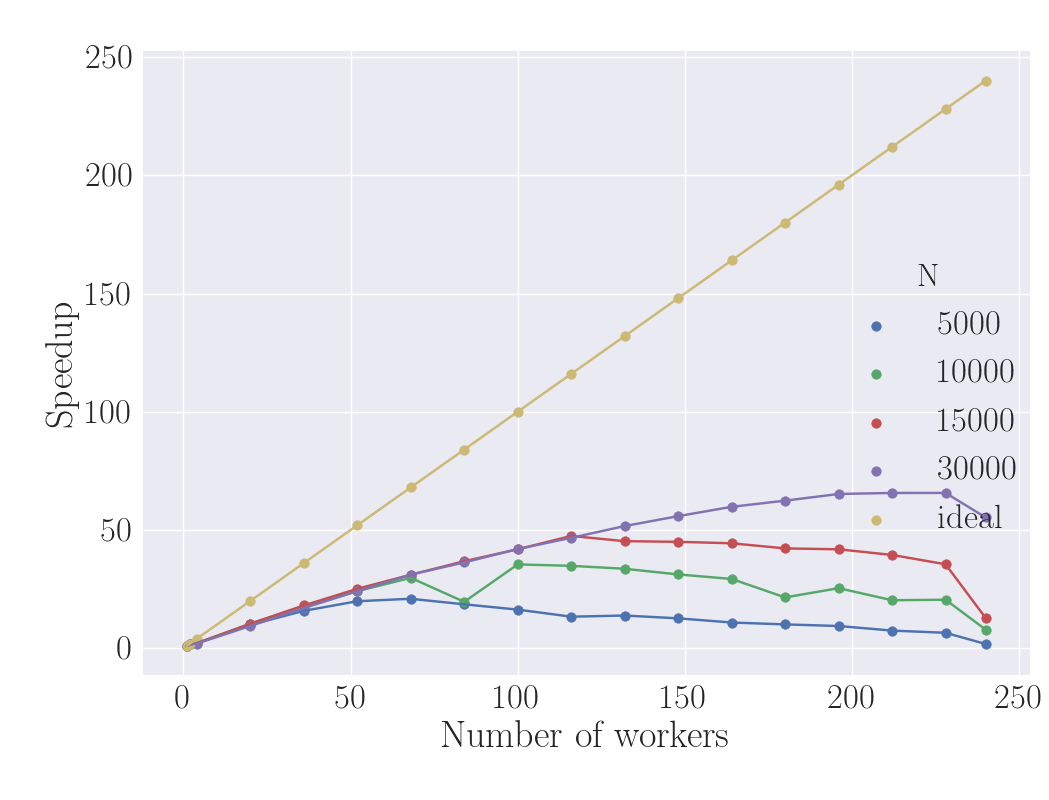
\includegraphics[width=\textwidth]{../graphs/graph_ff_mic_s}
		\caption{Speedup graph.}
		\label{fig:ff_mic_s}
	\end{subfigure}
	\begin{subfigure}[b]{0.3\textwidth}
		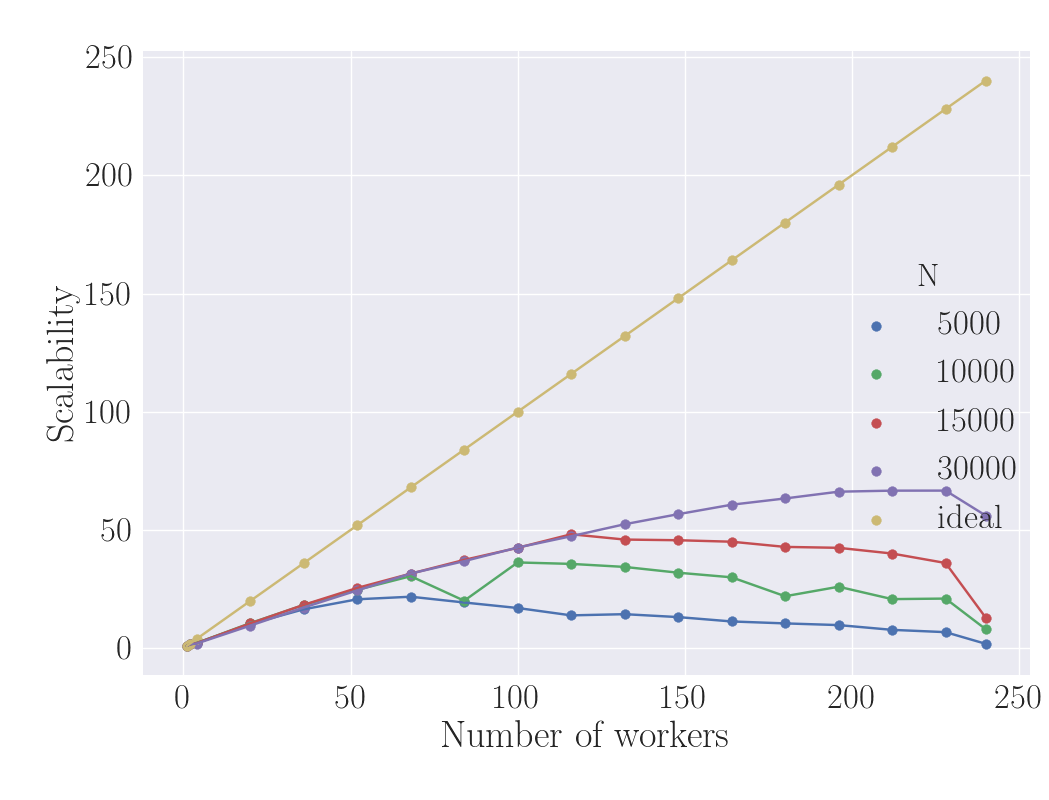
\includegraphics[width=\textwidth]{../graphs/graph_ff_mic_scalab}
		\caption{Scalability graph}
		\label{fig:ff_mic_scalab}
	\end{subfigure}
	\begin{subfigure}[b]{0.3\textwidth}
		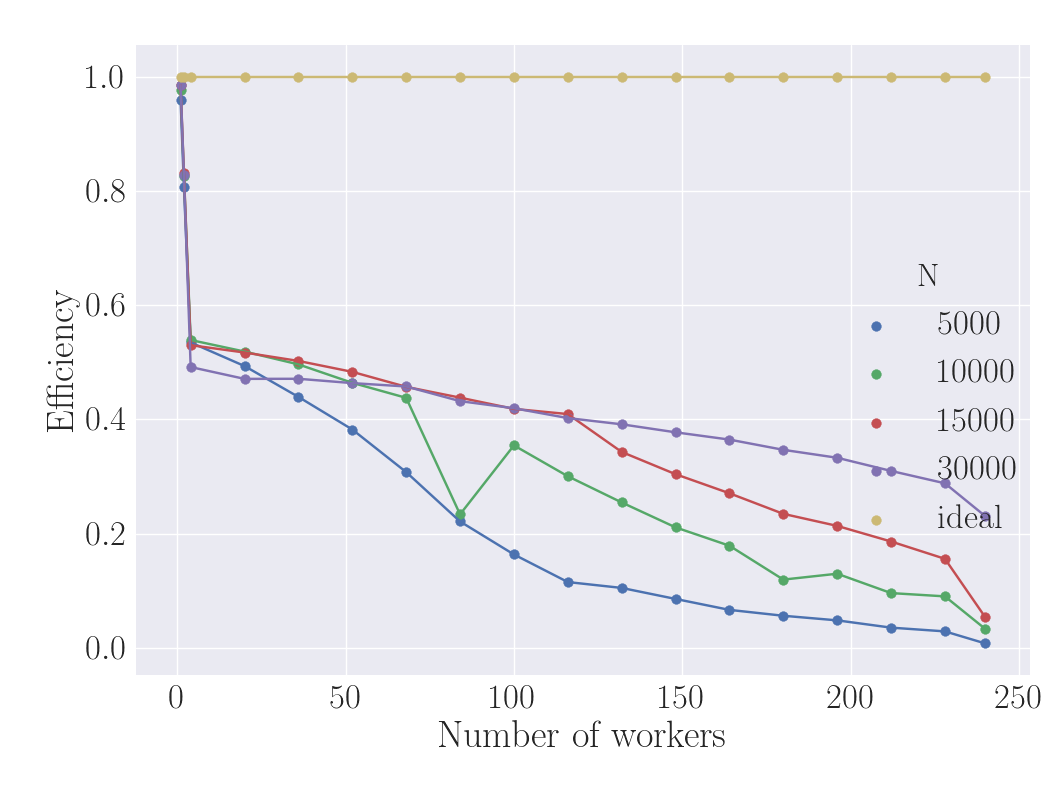
\includegraphics[width=\textwidth]{../graphs/graph_ff_mic_eff}
		\caption{Efficiency graph}
		\label{fig:ff_mic_eff}
	\end{subfigure}
	\caption{Graphs of different performance measures  on the Xeon Phi co-processor using FastFlow. $N \in \{ 5000, 10000, 15000, 30000\}$}
	\label{fig:ff_mic}
\end{figure}
~
\begin{figure}[h]
	\centering
	\begin{subfigure}[b]{0.3\textwidth}
		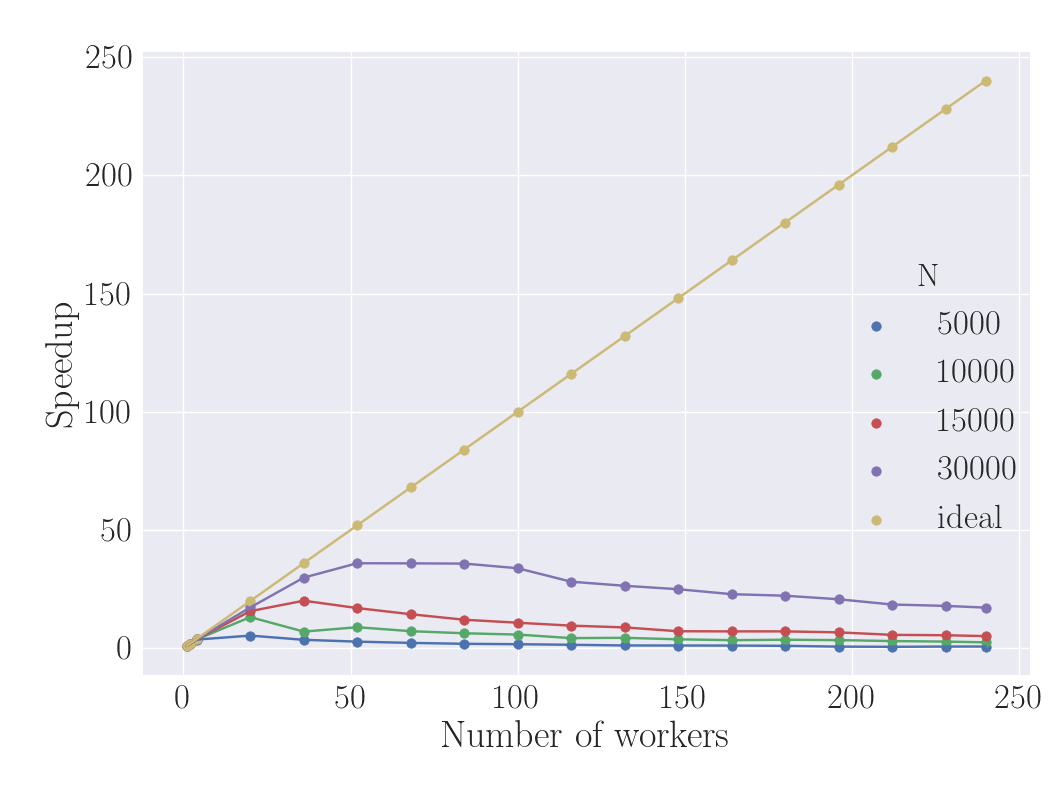
\includegraphics[width=\textwidth]{../graphs/graph_th_mic_s}
		\caption{Speedup graph.}
		\label{fig:th_mic_s}
	\end{subfigure}
	\begin{subfigure}[b]{0.3\textwidth}
		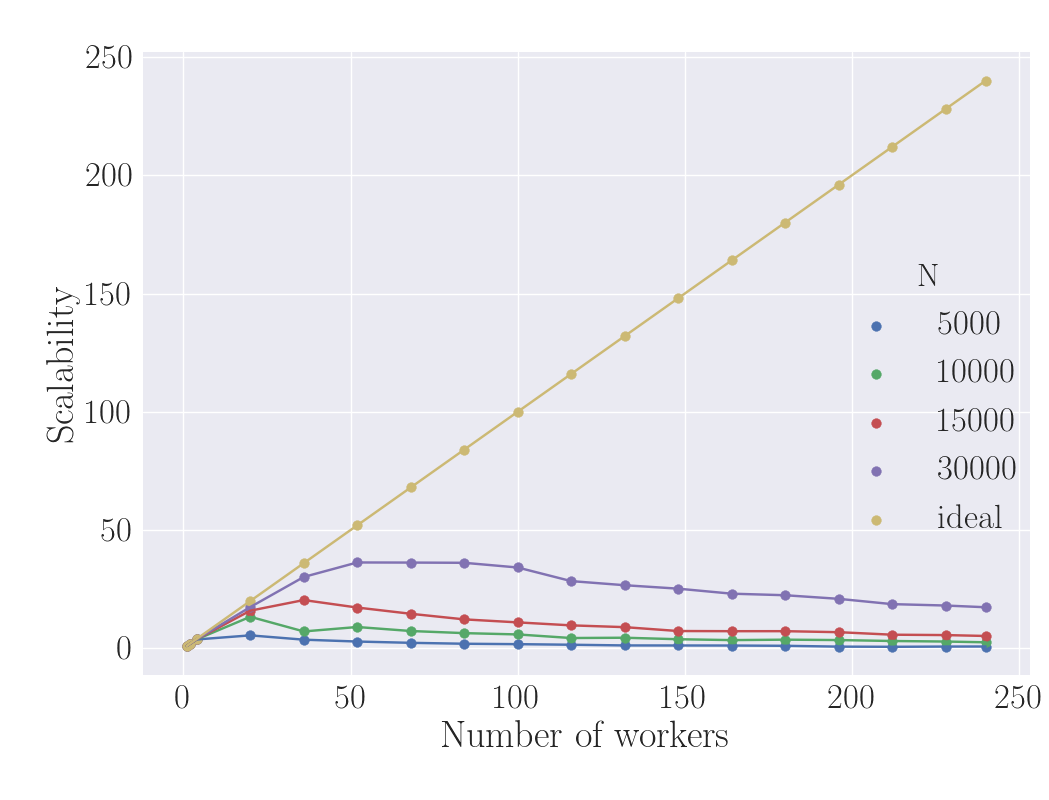
\includegraphics[width=\textwidth]{../graphs/graph_th_mic_scalab}
		\caption{Scalability graph}
		\label{fig:th_mic_scalab}
	\end{subfigure}
	\begin{subfigure}[b]{0.3\textwidth}
		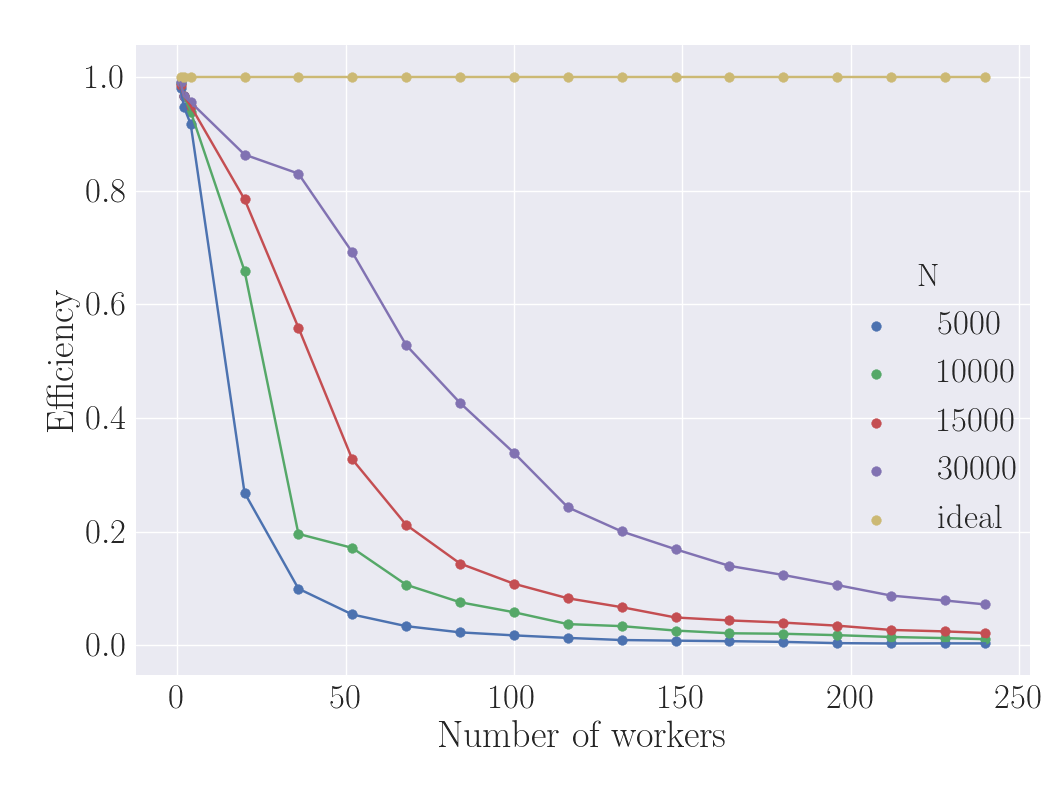
\includegraphics[width=\textwidth]{../graphs/graph_th_mic_eff}
		\caption{Efficiency graph}
		\label{fig:th_mic_eff}
	\end{subfigure}
	\caption{Graphs of different performance measures  on the Xeon Phi co-processor using C++11 threads. $N \in \{ 5000, 10000, 15000, 30000\}$}
	\label{fig:th_mic}
\end{figure}

Figure~\ref{fig:ff_mic} and Figure~\ref{fig:th_mic} respectively report the results of the execution of the FastFlow and C++11 thread implementation on the Xeon Phi co-processor.
As above none of the measured metrics adhere to the ideal curve.

In this case, on the other hand, bigger values of $N$ led to better performance metrics since the the time spent in setting up workers and in the barrier became smaller w.r.t.\ effective time of computation.
Also, in this case (up to $N = 30000$) cache coherence probably were not a bottleneck, since the cache size of the Xeon Phi is bigger than the one on the Xeon CPU.

Table~\ref{tab:res0} and Table~\ref{tab:res1} show, for each size $N$ of the system, the best configuration in term of minimal latency for the FastFlow and C++11 thread implementations, along with latency for the sequential implementation.

Note also that (most) of the best configurations use a number of workers smaller than the number of contexts, this is due to the fact that usually one context is used for orchestration.
\begin{table}[h]
	\centering
	\begin{tabular}{clcccc}  
		\toprule
		& & \multicolumn{2}{c}{\textbf{$N = 5000$}} & \multicolumn{2}{c}{\textbf{$N = 10000$}}\\
		\midrule
		& & \textbf{Xeon CPU} & \textbf{Xeon Phi} & \textbf{Xeon CPU} & \textbf{Xeon Phi}\\
		\cmidrule{3-6}		
		\textbf{Sequential} & $L_{seq}$ (\si{s}) & $0.055928$& $1.054620$ & $0.118950$& $0.782633$\\
		\midrule
		\textbf{FastFlow} & $L_1$ (\si{s}) & $0.064616$ & $0.209478$ & $0.255854$ & $0.800839$\\
		& $L_{w_{best}}$ (\si{s}) & $0.007958$ & $0.009615$ & $0.028755$ & $0.022076$\\
		& $w_{best}$ & $12$ & $68$ & $12$ & $100$\\
		\midrule
		\textbf{Thread} & $L_1$ (\si{s})& $0.064908$ & $0.205056$ & $0.255311$ & $0.791644$\\
		& $L_{w_{best}}$ (\si{s})& $0.012583$ & $0.037514$ & $0.045068$ & $0.059418$\\
		& $w_{best}$ & $16$ & $20$ & $16$ & $20$ \\
		\bottomrule
	\end{tabular}
	\caption{Best configurations in terms of minimal latency for FastFlow and C++11 thread implementations. 
		Here the number of workers that minimizes the latency is denoted by $w_{best}$, latency with $w$ workers as $L_w$, sequential latency as $L_{seq}$. ($N = 5000$ and $N=10000$)}
	\label{tab:res0}
\end{table}
~
\begin{table}[h]
	\centering
	\begin{tabular}{clcccc}  
		\toprule
		& & \multicolumn{2}{c}{\textbf{$N = 15000$}} & \multicolumn{2}{c}{\textbf{$N = 30000$}}\\
		\midrule
		& & \textbf{Xeon CPU} & \textbf{Xeon Phi} & \textbf{Xeon CPU} & \textbf{Xeon Phi}\\
		\cmidrule{3-6}		
		\textbf{Sequential} & $L_{seq}$ (\si{s}) & $0.261870$& $1.716810$ & $1.054620$& $6.797150$\\
		\midrule
		\textbf{FastFlow} & $L_1$ (\si{s})& $0.574178$ & $1.741540$ & $1.325130$ & $6.887530$\\
		& $L_{w_{best}}$ (\si{s})& $0.063033$ & $0.036150$ & $0.322207$ & $0.103486$\\
		& $w_{best}$ & $12$ & $116$ & $8$ & $228$\\
		\midrule
		\textbf{Thread} & $L_1$ (\si{s})& $0.571200$ & $1.740340$ & $1.783050$ & $6.861650$\\
		& $L_{w_{best}}$ (\si{s})& $0.098026$ & $0.085337$ & $0.429399$ & $0.189059$\\
		& $w_{best}$ & $16$ & $36$ & $16$ & $52$ \\
		\bottomrule
	\end{tabular}
	\caption{Best configurations in terms of minimal latency for FastFlow and C++11 thread implementations. 
		Here the number of workers that minimizes the latency is denoted by $w_{best}$, latency with $w$ workers as $L_w$, sequential latency as $L_{seq}$. ($N = 15000$ and $N=30000$)}
	\label{tab:res1}
\end{table}